\documentclass[sigconf]{acmart}

\usepackage{booktabs} % For formal tables

\settopmatter{printacmref=false} % Removes citation information below abstract
\renewcommand\footnotetextcopyrightpermission[1]{} % removes footnote with conference information in first column
\pagestyle{plain} % removes running headers

\begin{document}
\title{Teaching Big Data and Open Source Software\\
  on Chameleon Cloud}


\author{Gregor von Laszewski, Geoffrey C. Fox}
\affiliation{%
  \institution{Indiana University, Smith Research Center, 2805 E 10th
    St, Bloomington, Indiana, 47408}
}
\email{laszewski@gmail.com}


\begin{abstract}
  Project CH-818664, KVM: This paper reports on the experience that we
  gained form using chameleon cloud as part of a course on Big Data
  and Open Source Software. The course had 62 registered users and
  used 91\% of its allocation with 18195 SUs. The course studies
  software used in many commercial activities related to Big Data. The
  backdrop for course contains more than 370 software subsystems from
  which the students can select. Chameleon cloud was used by the
  students to conduct a course project that included the creation of a
  reproducible big data computational infrastructure with DevOps, as
  well as the execution of an application in this infrastructure. A
  rich variety of 31 projects were conducted. The result of the
  project with its 31 projects is published in an online class
  report. We report on success and challenges of chameleon cloud as
  used in classes. Chameleon Cloud provided the compute resources to
  make this class possible.
\end{abstract}

\keywords{Cloudmesh, Chameleon Cloud, Big Data }


\maketitle

\section{Introduction}

As part of a graduate course at Indiana University that was offered to
online and residential students Chameleon cloud was used as one of the
major compute resources for the class. The course studied software
used in many commercial activities related to Big Data. The backdrop
for course contains more than 370 software subsystems that have been
studied in collaboratively in class. The software
architecture represented by this collection has been discused and work
towards identifying best practices to deploy, access and interface
with them has been conducted. Topics of this class included:

\begin{enumerate}
\item The cloud computing architecture underlying open source big data
  software and frameworks that contrast them to high performance
  computing.
\item Analysis of software as part of an architecture with its
  different layers covering broad functionality and rationale for each
  layer.
\item Identification on how to create and replicate software
  environments combining cloud and DevOps technologies.
\item The main activity of the course included building a significant
  project using multiple complex big data subsystems to create a reproducible
  big data software stack combined with user code and data. 
\end{enumerate}

Topics taught in this class are therefore highly relevant for industry
as it not only exposes students to theoretical concepts with the topic
of big data, but also through practice while having access to clouds
and making them usable through DevOps and collaborative code
experiences. Students were using cloudmesh client
\cite{www-cloudmesh-client} making it possible to easily execute the code on
multiple different clouds and enabling comparative benchmark studies. Figure
\ref{F:course} illustrates that we pursued the theoretical and
practical components of this course in parallel.

\begin{figure}[htbp]
\centering
\fbox{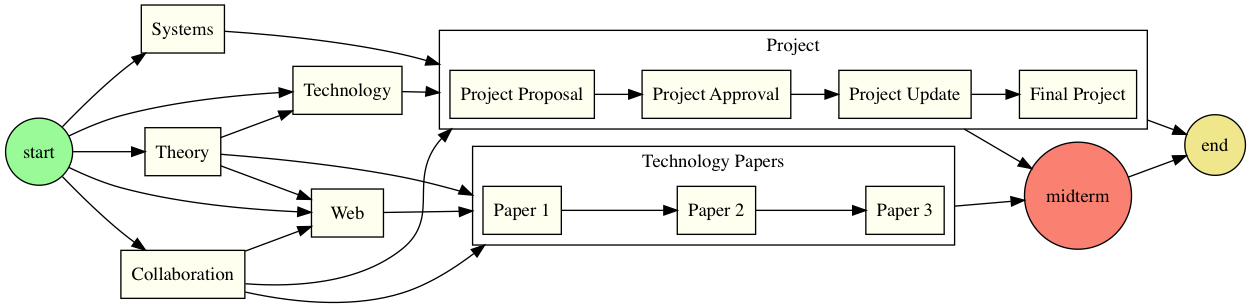
\includegraphics[width=\linewidth]{course.png}}
\caption{Course Tracks}
\label{F:course}
\end{figure}


\section{Cloud Usage}

The course had 62 registered users and used 91\% of its allocation
with 18195 SUs.  From 31 projects, 27 of them were completed while the other
4 are still being worked on. As the chameleon cloud allocation for
this project expires on July 31, we will have to apply for an extension.
Furthermore, we will run out of compute time for the outstanding
projects so we need to ask for an increase in the allocation.

In addition to Chameleon cloud, we also used Jetstream and the
FutureSystems cloud. Adding these clouds was essential to obtain
comparisons of chameleon cloud to other clouds.

\section{Projects}

The projects conducted as part of this class contained three major
portions. First, students had to design a software stack that relates
to big data and uses DevOps methods using {\it ansible} to create a
reproducible cyber infrastructure. This infrastructure had than to be
replicated on other clouds if the project was conducted in a
team. Chameleon cloud was recommended to be used as the default
cloud. Only after the projects were executable on chameleon other
clouds were allowed to be used.  A detailed report of all projects is
available online \cite{www-las-i524-sp17}. To provide an overview of
the richness of the projects we provide here a list of the titles:

\begin{itemize}

\item Remotely Deploying, Visualizing and Controlling a Robot Swarm with ROS
and Cloudmesh 

\item Charge Detection Mass Spectrometry

\item Automated Sharded MongoDB Deployment and Benchmarking for Big Data Analysis

\item Music Predictive Analysis Project based on Lyrics

\item Deploying CouchDB Cluster

\item Analysis of USGS Earthquake Data

\item Twitter sentiment analysis of the Affordable Care Act in 2017

\item Detection of street signs in videos in a robot swarm 

\item Analysis of H-1B Temporary Employment-Based in Data Science Occupation

\item On-line advertisement click prediction

\item Flight Data Analysis Using Big Data Tools

\item Real-time Analysis and Visualization of Twitter data

\item Aviation Data Analysis Using Apache Pig

\item Detecting Stop Signs in Images and Videos in a Robot Swarm

\item Using Hadoop and Spark for Big Data Analytics: Predicting Readmission of Diabetic patients

\item Analysis Of People Relationship Using Word2Vec on Wiki Data

\item Amazon Web Services Cloudmesh Extension

\item Deploying a spam message detection application using R over Docker and Kubernetes

\item Big data Visualization with Apache Zeppelin

\item Cloudmesh Docker Extension

\item Deployment of Vehicle Detection application on Chameleon clouds

\item Head Count Detection Using Apache Mesos

\item Optical Character Recognition

\item Weather Data Analysis

\item Analysis of Airline delays data using Spark and HDFS

\item Deployment and performance analysis of a Storm cluster on various cloud environments 

\item Predicting Customer Churn Using Apache Spark Machine Learning 

\end{itemize}

\section{Experimental configuration}

Conducting a class with many students provides its unique challenges
which are amplified when complex software and complex projects are
required as part of the course. Hence, it is worth while to analyze as
part of Chameleon Clouds mission how to support such educational projects. We
will outline here some challenges and important contributions of our
activities to Chameleon Cloud.

\subsection{Resource Requirements}

Based on our rich experience with other clouds, such as FutureGrid
and FutureSystems, we knew that the class projects needed to be limited
in order to stay within 20K SUs. Thus we limited each project team to
utilize only 3 virtual machines as part of their project and making
sure that the application and data sizes were small in nature while
limiting the possible analysis. Furthermore, we asked the students to
stop their machine when not in use.

Hence we have for cloud usage the requirement, to start and stop
virtual machines while not encountering too much penalties as this
supported the goal of teaching DevOps. Naturally, this requires not
only a ``perfect'' application to be executed, but to support the
process of developing the software stack that can be reproduced and
potentially executed on other clouds. Hence the charge rate of
starting and stopping VMs must be small.

Lessons learned: In contrast to jetstream chameleon cloud provided a
reasonable charge rate that did not impact the overall allocation
adversely. However, we found that it would be useful to have a more
clear and prominent description of the charge formula published in
order to educate the students better of prudent usage. Just as
Chameleon Cloud Jetstream did also not have this information
published.  After our allocation on jetstream (which was much smaller)
expired, we found we were charged on jetstream a full hour every time
a students started a VM. This charge seems unreasonably high for our
class goals and we need to discuss with jetstream management changes
to it. This information was not available to us when we formulated the
allocation proposal.  As students started and restarted VMs this
several times per hour on jetstream we ran out of SUs quickly. Our
allocation was renewed after several interactions while initially
being declined with the comment we need to provide justification and
performance analysis. Naturally if you are in a middle of an
educational project that has not yet produced this result such request
can not be completed. Only after we contacted the excellent Jetspeeds
technical team directly via phone this situation was rectified by
switching off accounting for this project to enable continued use. We
found that the allocation process for educational projects in XSEDE
does not include the important aspect to easily renew an allocation if
one runs out of node hours. We found that chameleon cloud has a better
charge rate for starting and stopping VMs as any research cloud should
have, making jetstream less desirable for research classes and
encourages resource hogging for an hour and not allowing for flexible
development of utilizing VM startup. We hope that chameleon cloud will
continue their charge model and make sure that start of VMS is not
taxed at all.

Overall we also found that in contrast to FutureGrid both clouds do
not offer easily sufficient access to real time monitoring data going
beyond just the hours run by a VM but also including time for starting
and stopping VMs. 

\subsection{Capability Requirements}

Based on our current experience we found that offering bare-metal as part of a
class such as the one described is not feasible due to the lack of
experience of most of the students. The risk to expose security issues
is far to high in order to justify that a class such as the one we
offered would have access to bare-metal. Please note that the authors
are pioneered offering bare metal services on clouds
\cite{las08federated-cloud}. For this class the VM model is much more
suitable. 

\subsection{Capacity Requirements}

At time we noticed that chameleon cloud was too busy and not all
request could be fulfilled. Thus, it would have helped to have access
to a queuing system that allows scheduling of vm execution. However,
during development waiting is naturally not a good idea and most
students recognized when chameleon was too busy or had other
interruptions. 

\subsection{Monitoring Requirements}

Due to the many users in this project it is not sufficient to just
provide the overall charge. It is important that the project managere
can see the individual charges of all users. This service is
conveniently offered by Futuresystems and we propose reintegration
into chameleon cloud. We also noticed that students overlooked the
outage notice and a much more clear communication of the status of the
coud on its front page of the portal must be available. We again refer
back to FutureGrid that provided such features.

\subsection{Features offered by Chameleon Cloud}

As part of this class we used direct access to the REST interface for
OpenStack using virtual machines. The horizon interface was used by
some students to just make sure that the VMs were started and had the
correct security groups associated. However, the overwhelming majority
of the students used cloudmesh client that conveniently provides this
information not just for one cloud but many clouds from the
commandline. Furthermore, almost all vm management was conducted via
the cloudmesh client. This convenient mechanism was superior to the
native client offered by OpenStack. GUIs were inconvenient including
CyVerse and Horizon as they do not offer easy scriptability while
applying it to multi-clouds. 

\subsection{New software created}

As part of this class we improved the cloudmesh client software
\cite{www-cloudmesh-client}\cite{www-cloudmesh-cmd5}
\cite{www-cloudmesh-rest} that was essential to the success of the
class.

In addition, many DevOps deployments for deploying virtual clusters
based on hadoop, docker swarm, kubernetes and others have been
developed and are available as part of the open source class repository
including the applications and documentation on how to deploy and run
them.

\subsection{User Management}

It is clear that the class has a significant user management
challenge. We found that the management for large project could be
improved and inspiration from FutureSystems/Grid could be utilized to
improve the ease in which project membership could be managed.

The biggest issue however we had was with the user management provided
across different clouds and high performance compute infrastructure
such as XSEDE. As it turns out a broken process is offered to users
that have accounts on one or more resources that provide user
management through the centralized user management service for XSEDE,
chameleon and jetstream. After many tickets it was not clear to us if
the problem has generally been solved, or if it was just solved for
the users that ran into the issue. We observed that in certain cases,
where users have existing accounts on one or more resources, it leads
to the situation where some users could not access one ore more of the
systems. Obviously the students with this issue could not identify if
they are effected as they thought their account approval is in process
and they need to wait. Only after all other class members were well
into their project execution it became clear that the user
accountmanagement had an issue. Consequently, we found that the
process was broken.

Based on our experience with other clouds and infrastructure, students
have no issue remembering multiple account names and passwords for
different services (this is naturally the nature of the cloud, they
have Google, Microsoft, box, ...), but they have an issue of an
account service trying to offer SSO and ease of account management
does not 100\% work. The students gave the recommendation that
Chameleon cloud fixes this issue with the organization that offers
this service to chameleon cloud.

\subsection{Performance Comparison}

We have conducted detailed performance studies on applications
comparing chameleon cloud, jetstream and FutureSystems. While
FutureSystems is an older cloud and can not compete on a vm level on
speed, it still provides a reliable basis for running VMs. The speed
between Chameleon Cloud and jetstream VMs is very similar. We ran in
both clouds via cloudmesh. Jetstream was accessed in friendly user
mode and experienced at times network outages which we expected. We
had good communication with the technical group to jetstream whenever
we contacted the directly by phone. In general chameleon cloud was a
very reliable cloud and due to the staff support at University of
Chicago we were able to overcome any reported issue quickly.

\section{Conclusion}

We were able to support 62 students as part of the class using
chameleon cloud as the main resource. The experience was so good that
we intend to apply again for vm usage of another class in the fall. A
significant amount of software was developed as part of this class
while using DevOps and making the results freely available. Cloudmesh
client allowed the class to easily switch between chameleon jetstream
and FutureSystems, thus in a case of an outage they could easily
continue their work elsewhere. In fact we believe that cloudmesh
client was one of the reasons for the class to be possible and easily
accessible to the students. It also allowed performance studies
between the clouds. A full report with all completed projects is
available online. The biggest issue we had were the bugs in the SSO
framework offered between XSEDE, chameleon cloud and jetstream.


\bibliographystyle{ACM-Reference-Format}
\bibliography{references} 

\end{document}

